\section{Interprocedural Profiling}

The first contribution we present in this thesis is an {\em interprocedural} technique for identifying the calling context that are most frequently encountered across function invocations at run-time. We show that the traditional approach for constructing a {\em Calling Context Tree} (CCT) might not be sustainable for real-world applications, as their CCTs often consist of tens of millions of nodes, making them difficult to analyze and also hurting execution time because of poor access locality. We thus introduce a novel data structure, the {\em Hot Calling Context Tree} (HCCT), in the spectrum of representations for interprocedural control flow. The HCCT is defined as the subtree of the CCT containing only its most visited nodes, which we call {\em hot}, along with their ancestors, and can be constructed independently of the CCT using fast, space-efficient algorithms for mining frequent items in data stream.

\subsection{Motivation and Contributions}
The dynamic {\em calling context} of a routine invocation is defined as the sequence of functions that are concurrently active on the run-time stack. A calling context leads to an exact program location, as it corresponds to the sequence of un-returned calls from a program’s root function to the routine invocation it is associated with.

Context-sensitive profiling information provides valuable information for program understanding, performance analysis, and runtime optimizations. Previous works demonstrated its effectiveness for tasks such as residual testing~\cite{PavlopoulouY99,Vaswani07}, function inlining~\cite{Chang92}, statistical bug isolation~\cite{Feng03,Liblit03}, performance bug detection~\cite{Nistor13}, object allocation analysis~\cite{Nethercote07}, event logging~\cite{Zhang06}, or anomaly-based intrusion detection~\cite{Bond07}.
% this is a sync with PCCE paper
Calling-context information can also be employed in unit test generation~\cite{Villazon09}, testing of sensor network applications~\cite{Lai08}, and reverse engineering of protocol formats~\cite{Lin08}.

\begin{table}[ht]
%\centering
\begin{center}
\begin{tabular}{|l|r r r r|}
\hline
Application & $|$Call graph$|$ & Call sites & $|$CCT$|$ & $|$Call tree$|$\\
\hline
amarok & 13\,754 & 113\,362 & 13\,794\,470 & 991\,112\,563 \\
ark & 9\,933 & 76\,547 & 8\,171\,612 & 216\,881\,324 \\
audacity & 6\,895 & 79\,656 & 13\,131\,115 & 924\,534\,168 \\
bluefish & 5\,211 & 64\,239 & 7\,274\,132 & 248\,162\,281 \\
dolphin & 10\,744 & 84\,152 & 11\,667\,974 & 390\,134\,028 \\
firefox & 6\,756 & 145\,883 & 30\,294\,063 & 625\,133\,218 \\
gedit & 5\,063 & 57\,774 & 4\,183\,946 & 407\,906\,721 \\
ghex2 & 3\,816 & 39\,714 & 1\,868\,555 & 80\,988\,952 \\
gimp & 5\,146 & 93\,372 & 26\,107\,261 & 805\,947\,134 \\
gwenview & 11\,436 & 86\,609 & 9\,987\,922 & 494\,753\,038 \\
inkscape & 6\,454 & 89\,590 & 13\,896\,175 & 675\,915\,815 \\
oocalc & 30\,807 & 394\,913 & 48\,310\,585 & 551\,472\,065 \\
ooimpress & 16\,980 & 256\,848 & 43\,068\,214 & 730\,115\,446 \\
oowriter & 17\,012 & 253\,713 & 41\,395\,182 & 563\,763\,684 \\
pidgin & 7\,195 & 80\,028 & 10\,743\,073 & 404\,787\,763 \\
quanta & 13\,263 & 113\,850 & 27\,426\,654 & 602\,409\,403 \\
sudoku & 5\,340 & 49\,885 & 2\,794\,177 & 325\,944\,813 \\
vlc & 5\,692 & 47\,481 & 3\,295\,907 & 125\,436\,877 \\
%\hline
botan & 3\,388 & 27\,114 & 308\,550 & 26\,272\,804\,980 \\
cairo-perf-trace & 1\,408 & 3\,696 & 137\,920 & 15\,976\,619\,734 \\
crafty & 107 & 516 & 36\,434\,095 & 10\,403\,074\,070 \\
fhourstones & 18 & 32 & OOM & 39\,272\,563\,944 \\
gobmk & 1\,133 & 4\,049 & OOM & 21\,909\,088\,291 \\
ice-labyrinth & 2\,335 & 8\,050 & 2\,160\,052 & 1\,637\,076\,406 \\
mount-herring & 2\,318 & 8\,269 & 3\,733\,120 & 3\,311\,257\,932 \\
overworld & 14\,173 & 50\,394 & 3\,774\,937 & 4\,112\,679\,880 \\
scotland & 13\,932 & 51\,206 & 1\,813\,368 & 5\,982\,612\,379 \\
sjeng & 57 & 221 & OOM & 28\,370\,207\,811 \\
\hline
\end{tabular}
\vspace{4mm}
\caption{\label{tab:CCTsize} Number of nodes of call graph, call tree, calling context tree, and number of distinct call sites for different applications. OOM stands for {\em Out Of Memory} (i.e., the CCT is too large to be constructed in main memory on a 32-bit architecture). %Game PlanetPenguin Racer has been run on two different courses (mount-herring and ice-labyrinth). Similarly, game SuperTuxKart has been run on tracks overworld and scotland.
}
\end{center}
\end{table}
\vspace{-8mm}

\ifauthorea{\newline}{}

\mynote{Add reference to related work section for the CCT}
Calling context trees (CCTs) offer a compact representation for context-sensitive information. In fact, a CCT yields a more accurate profile than a {\em call graph} (which can sometimes drive to misleading conclusions~\cite{Ponder88, Spivey04}) in a space that is typically several orders of magnitude smaller than the one required to maintain a {\em call tree}. Many techniques have also been proposed over the years to reduce the overhead for its construction.
%, by trading accuracy for performance.

However, even CCTs may be very large and difficult to analyze in several applications~\cite{Bond07,Zhuang06}; their sheer size might also hurt execution time, because of poor access locality during construction and query. As an example, we report in \mytable\ref{tab:CCTsize} numbers collected for short usage sessions of off-the-shelf Linux applications and for benchmarks from popular suites. Under the optimistic assumption that each CCT node requires 20 bytes for its representation on a 32-bit architecture\footnote{From maintaining the routine ID, the call site, and the metric using {\tt int} fields, along with two pointers for a first-child, next-sibling representation. Previous works~\cite{Ammons97,Spivey04} use larger nodes.}, nearly 1 GB of memory is needed just to maintain OpenOffice Calc's 48-million-node CCT.

In a performance profiling scenario, only the most frequent contexts are of interest, as they represent the hot spots to which optimizations must be directed. As observed in~\cite{Zhuang06}: ``Accurately collecting information about hot edges may be more useful than accurately constructing an entire CCT that includes rarely called paths.'' \myfigure\ref{fig:hcct-skewness} shows that, for different applications, only a small fraction of contexts are hot: in conformance with the Pareto principle, nearly 90\% of routine calls take place in only 10\% of contexts. The skewness of function-call distribution suggests that space could be greatly reduced by keeping information about hot contexts only and discarding on the fly contexts that are likely to be cold, i.e., to have low frequency.

\ifdefined\noauthorea
\begin{figure}[hb]
\begin{center}
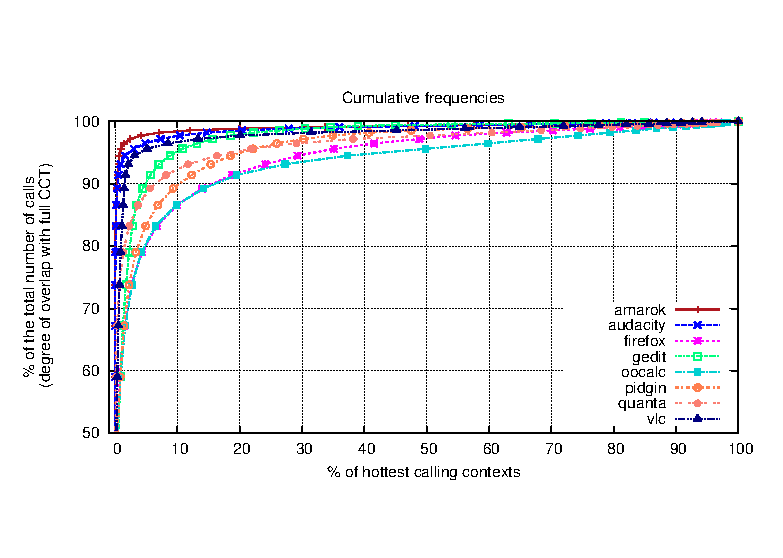
\includegraphics[width=0.95\columnwidth]{figures/hcct-skewness/hcct-skewness.eps}
\caption{\protect\label{fig:hcct-skewness} Skewness of calling contexts distribution on a representative subset of applications. For instance, in {\tt oocalc}, 10\% of the hottest calling contexts account for more than 86\% of all routine calls.
}
\end{center}
\end{figure}
\fi

Lorem ipsum...
%~\cite{}

%Context-sensitive profiling provides 
%These algorithms allow us to distinguish between hot and cold context on-the-fly, and we show both theoretically and experimentally that for collected metrics the HCCT achieves a similar precision as the CCT in a space that is several orders of magnitude smaller. We show on prominent benchmarks that our implementation, shipping as a plugin for the \gcc\ compiler, incurs a slowdown competitive with the \gprof\ profiler while collecting much finer-grained profiles.

\subsection{Approach}

\subsection{Algorithms}

\subsection{Implementation}

\subsection{Comparison with Related Work}

\subsection{Discussion}
